\documentclass{article}

\usepackage[preprint]{neurips_2024}

% ---------------------------------------------------------
% PACKAGES
% ---------------------------------------------------------
\usepackage{times}
\usepackage{graphicx}
\usepackage{hyperref}
\usepackage{amsmath}
\usepackage{amssymb}
\usepackage{enumitem}
\usepackage{tikz}
\usetikzlibrary{positioning}
\usepackage{listings}
\usepackage{xcolor}

\lstset{
  basicstyle=\ttfamily\small,
  breaklines=true,
  frame=single,
  backgroundcolor=\color{gray!10},
}

% ---------------------------------------------------------
% TITLE
% ---------------------------------------------------------
\title{
Convergence IO: A Local-First Runtime for\newline
Provider-Aware Routing and Audit-Traceable AI Interaction
}

\author{
Alex Place \\
\texttt{github.com/alex-place}
}

\begin{document}

\maketitle

% ---------------------------------------------------------
% ABSTRACT
% ---------------------------------------------------------
\begin{abstract}
We describe Convergence IO, a local-first runtime architecture that routes user
queries across heterogeneous language-model providers (cloud APIs, local
inference endpoints) while maintaining append-only audit traces and structured
caching. The system is deployed within ORION, a personal dream-journaling and
symbolic-interaction environment. We present the design goals---provider-aware
routing, local data ownership, and structured provenance logging---and report on
the engineering trade-offs encountered during deployment: external API privacy
leakage, the lack of formal routing guarantees, and the absence of quantitative
reliability metrics. We do not claim empirical improvements over baselines; this
paper is a systems description intended to motivate community discussion on
capability-transparent, user-owned AI infrastructure.
\end{abstract}

% ---------------------------------------------------------
% 1. INTRODUCTION
% ---------------------------------------------------------
\section{Introduction}

Modern AI systems increasingly rely on heterogeneous collections of large
language models (LLMs), local inference engines, and specialized symbolic
components. While these systems achieve impressive task performance, users
lack transparency into which model processes their data, whether a cheaper or
more capable alternative was available, and whether their inputs are retained
by third-party providers.

This paper introduces Convergence IO, a local-first runtime that addresses these
concerns through three concrete design goals:
\begin{enumerate}[label=(\arabic*)]
    \item \textbf{Provider-aware routing:} the system maintains real-time
    health state for each available provider and routes requests accordingly.
    \item \textbf{Local data ownership:} conversation histories, dream
    journals, and operator notes are stored as append-only JSONL files on the
    user's machine.
    \item \textbf{Structured provenance logging:} every model interaction is
    recorded with timestamp, provider identifier, and message payload, producing
    a complete, locally auditable trace.
\end{enumerate}

The architecture is deployed within ORION, a personal dream-journaling
application that integrates neural generative models with symbolic interaction
mechanisms such as the ``3 Door Game.'' ORION serves as a real-world testbed
for evaluating the practical challenges of user-owned AI infrastructure.

\textbf{Scope and limitations.} This paper is a \emph{systems description}, not
an empirical study. We report on implementation choices, observed failure
modes, and open engineering questions. We do not present controlled experiments,
baselines, or quantitative superiority claims.

% ---------------------------------------------------------
% 2. BACKGROUND AND RELATED WORK
% ---------------------------------------------------------
\section{Background and Related Work}

\paragraph{LLM routing.} RouterBench~\cite{} and LLM-BLENDER~\cite{}
demonstrate that routing queries to the most appropriate model can improve
cost--quality trade-offs. These systems rely on benchmark datasets and
pre-trained routers. Convergence IO differs in that routing decisions are
heuristic, based on live provider health checks and user-configured fallbacks,
rather than learned from labeled data.

\paragraph{Local-first software.} The local-first software movement~\cite{}
advocates data ownership, offline capability, and peer-to-peer
synchronization. ORION stores all user data as local JSONL files and never
requires cloud persistence, though it optionally forwards chat messages to
external APIs for inference.

\paragraph{Provenance and audit.} W3C PROV~\cite{} and related standards
define formal models for provenance graphs. Convergence IO adopts a lightweight,
append-only JSONL log format rather than a full provenance ontology, trading
expressivity for implementation simplicity.

\paragraph{Privacy in personal AI.} On-device inference (e.g., Ollama,
llama.cpp) keeps data local but sacrifices model capability. Cloud APIs offer
stronger models but require sending user data to third parties. Convergence IO
currently leaks dream-journal text to external providers during chat; we
discuss this as an open limitation rather than a solved problem.

% ---------------------------------------------------------
% 3. SYSTEM OVERVIEW
% ---------------------------------------------------------
\section{System Overview}

ORION consists of four layers (Figure~\ref{fig:arch}):

\begin{enumerate}[label=(\arabic*)]
    \item \textbf{Frontend:} A single-page HTML/JS application
    (\texttt{dream-chat-orion.html}) that renders chat bubbles, handles SSE
    streaming, and provides offline fallback replies.
    \item \textbf{HTTP Server:} A Node.js server (\texttt{server.js},
    \texttt{cloud-server.js}, \texttt{render-server.js}) that exposes REST
    endpoints for chat, status, file serving, and action dispatch.
    \item \textbf{Routing Engine:} A Python module
    (\texttt{convergence\_io\_engine.py}) that implements tier-based provider
    selection, circuit breakers, and metrics collection.
    \item \textbf{Storage Layer:} JSONL files managed by a serializing file
    queue (\texttt{file-queue.js}) and a binary cache manager
    (\texttt{csf\_cache\_manager.py}) with CRC32 + SHA-256 integrity checks.
\end{enumerate}

\begin{figure}[h]
\centering
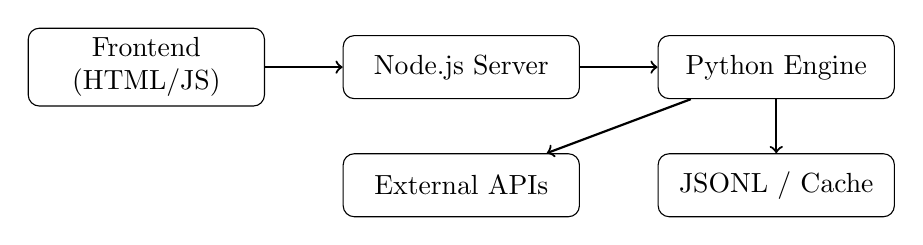
\begin{tikzpicture}[
    box/.style={draw, rounded corners, minimum width=3cm, minimum height=0.8cm, align=center},
    arrow/.style={->, thick}
]
\node[box] (fe) at (0,0) {Frontend\\(HTML/JS)};
\node[box] (srv) at (4,0) {Node.js Server};
\node[box] (eng) at (8,0) {Python Engine};
\node[box] (sto) at (8,-1.5) {JSONL / Cache};
\node[box] (api) at (4,-1.5) {External APIs};
\draw[arrow] (fe) -- (srv);
\draw[arrow] (srv) -- (eng);
\draw[arrow] (eng) -- (sto);
\draw[arrow] (eng) -- (api);
\end{tikzpicture}
\caption{Simplified architecture of Convergence IO / ORION.}
\label{fig:arch}
\end{figure}

% ---------------------------------------------------------
% 4. DESIGN AND IMPLEMENTATION
% ---------------------------------------------------------
\section{Design and Implementation}

\subsection{Provider-Aware Routing}

The routing engine maintains a registry of providers (Anthropic Claude, OpenAI,
Google Gemini, local Ollama). Each provider advertises a tier and a health
state. The engine selects providers in priority order; if the chosen provider
fails or returns an error, the engine falls back to the next tier.

Health is determined by:
\begin{itemize}
    \item A configurable timeout on API responses.
    \item Recent error-rate tracking via a sliding window.
    \item Explicit user overrides (e.g., forcing local-only mode).
\end{itemize}

We emphasize that this routing is \emph{heuristic}. There is no formal
guarantee that the selected provider is optimal for a given query, nor do we
learn routing policies from data. The system simply prefers healthier,
higher-tier providers and degrades gracefully.

\subsection{Local Storage and Audit Traces}

All user-visible state is stored as append-only JSONL files:
\begin{itemize}
    \item \texttt{data/conversations/garage-conversations.jsonl} --- chat
    history.
    \item \texttt{data/dream\_journal/dreams\_YYYY-MM.jsonl} --- dream entries.
    \item \texttt{data/operator-notes/notes.jsonl} --- operator feedback.
\end{itemize}

Writes are serialized through a per-file queue (\texttt{file-queue.js}) to
prevent interleaved JSONL corruption under concurrent HTTP handlers. Each line
is a self-contained JSON object; partial writes are recoverable by discarding
the final malformed line.

Provenance is limited to timestamp, provider identifier, and message payload.
We do not cryptographically sign records or build a Merkle tree; tampering is
possible by anyone with filesystem access. The goal is auditability (a complete
history exists) rather than integrity (the history is tamper-evident).

\subsection{Cache Integrity Layer (CSF)}

The Convergence Symbolic Format (CSF) cache manager
(\texttt{csf\_cache\_manager.py}) provides a binary key--value cache with:
\begin{itemize}
    \item TTL-based expiration (default 3600 seconds).
    \item CRC32 + SHA-256 integrity checks on each record.
    \item A Python decorator for caching function results.
\end{itemize}

We clarify that CSF is \emph{not} a sparse ternary matrix or symbolic-reasoning
substrate. It is a conventional cache with extra integrity checks. The name
``Symbolic Format'' is historical; the implementation is a key--value store.

A separate utility (\texttt{qutrit.js}) generates 12-character base-3
identifiers for dream entries, but this is not connected to the cache encoding.

\subsection{Tool Hooks and Safety Boundaries}

The \texttt{agent\_tool\_hooks.py} module implements pre- and post-call checks
around tool invocations: rate limiting, cache read/write, safety keyword
filtering, and retry logic. These are lightweight guardrails rather than formal
verification; a determined adversary with code access can bypass them.

\subsection{Deployment Modes}

ORION runs in three modes:
\begin{enumerate}[label=(\arabic*)]
    \item \textbf{Local:} Full read/write, PowerShell actions enabled,
    all APIs exposed on \texttt{localhost:4177}.
    \item \textbf{Cloud (read-only):} Most POST endpoints return
    \texttt{403 cloud\_read\_only}. Only chat streaming and dream creation are
    permitted; actions are disabled.
    \item \textbf{Render (static):} Serves public HTML and read-only status
    JSON. No write operations.
\end{enumerate}

Mode selection is compile-time (different entry points) rather than runtime
ACL-based. This is simpler but less flexible.

% ---------------------------------------------------------
% 5. OBSERVED LIMITATIONS AND OPEN QUESTIONS
% ---------------------------------------------------------
\section{Observed Limitations and Open Questions}

We report the following limitations candidly, as they motivate future work
rather than diminish the system's value.

\paragraph{Privacy leakage.} Chat messages and dream-journal text are sent to
external APIs (Anthropic, OpenAI, Google). The system is therefore \emph{not}
privacy-preserving in the formal sense; it is locally auditable but not
locally contained. Future work includes on-device inference for sensitive
queries and differential-privacy wrappers for cloud-bound data.

\paragraph{No formal routing guarantees.} Provider selection is heuristic. We
have not measured routing accuracy, cost savings, or quality degradation
relative to a single-provider baseline. A meaningful evaluation would require:
(a) a labeled dataset of query--provider--quality triples, (b) a cost model for
each provider, and (c) a user-study protocol. None of these currently exist.

\paragraph{Unbounded metrics growth.} The Python metrics collector
(\texttt{convergence\_io\_engine.py}) accumulates error and throughput counters
in unbounded dictionaries. Long-running processes will leak memory. These
structures should be replaced with ring buffers or TTL maps.

\paragraph{Path-traversal risk.} Static-file serving in
\texttt{server.js} and \texttt{render-server.js} uses
\texttt{path.resolve(...).startsWith(root)} as a directory guard. This is
vulnerable to case-mismatch attacks on Windows and symlink traversal on all
platforms. A safer guard uses \texttt{path.relative} and checks for
\texttt{..} prefixes.

\paragraph{Missing schema validation.} There are no formal JSON schemas for
conversation entries, dream records, or provider state. Data is parsed with
\texttt{JSON.parse} and validated ad-hoc, risking silent corruption.

\paragraph{Resource leaks.} The Python \texttt{ThreadPoolExecutor} is never
shut down, and spawned PowerShell processes have no timeout. Under repeated
creation or hung scripts, resources leak.

% ---------------------------------------------------------
% 6. CONCLUSION
% ---------------------------------------------------------
\section{Conclusion}

Convergence IO is a working local-first runtime that routes AI queries across
multiple providers while storing complete audit traces on the user's machine. It
demonstrates that a small, self-contained system can provide provider
awareness, local data ownership, and structured logging without requiring cloud
infrastructure or complex orchestration.

The system also illustrates the gap between aspiration and implementation:
``privacy-preserving'' becomes ``locally auditable but externally leaky'';
``capability-honest'' becomes ``heuristic routing with fallback''; and
``provenance-driven'' becomes ``append-only JSONL.'' We believe these honest
reductions are valuable contributions in their own right, because they define
clear, measurable next steps for the research community.

Future work includes formalizing provider-selection policies, adding
cryptographic integrity to audit logs, conducting user studies on routing
transparency, and exploring on-device inference for privacy-sensitive queries.

% ---------------------------------------------------------
% REFERENCES
% ---------------------------------------------------------
\bibliographystyle{plain}
% Placeholder --- real citations needed before submission.
\begin{thebibliography}{9}
\bibitem{routerbench} RouterBench: A Benchmark for Multi-LLM Routing.
\bibitem{llmblender} LLM-BLENDER: Ensembling Large Language Models with Pairwise Ranking and Fused Generation.
\bibitem{localfirst} Local-First Software: You Own Your Data, in Spite of the Cloud.
\bibitem{w3cprov} W3C PROV: The Provenance of Data.
\end{thebibliography}

\end{document}
